% !TEX TS-program = pdflatex
% !TEX encoding = UTF-8 Unicode

% This is a simple template for a LaTeX document using the "article" class.
% See "book", "report", "letter" for other types of document.

\documentclass[11pt]{article} % use larger type; default would be 10pt

\usepackage[utf8]{inputenc} % set input encoding (not needed with XeLaTeX)
\usepackage{listingsutf8}

%%% Examples of Article customizations
% These packages are optional, depending whether you want the features they provide.
% See the LaTeX Companion or other references for full information.

\usepackage{wrapfig}

%%% PAGE DIMENSIONS
\usepackage{geometry} % to change the page dimensions
\geometry{a4paper} % or letterpaper (US) or a5paper or....
% \geometry{margin=2in} % for example, change the margins to 2 inches all round
% \geometry{landscape} % set up the page for landscape
%   read geometry.pdf for detailed page layout information

\usepackage{listings}
\usepackage{color}

\definecolor{dkgreen}{rgb}{0,0.6,0}
\definecolor{gray}{rgb}{0.5,0.5,0.5}
\definecolor{mauve}{rgb}{0.58,0,0.82}

\lstset{frame=tb,
  language=C,
  aboveskip=3mm,
  belowskip=3mm,
  showstringspaces=false,
  columns=flexible,
  basicstyle={\small\ttfamily},
  numbers=none,
  numberstyle=\tiny\color{gray},
  keywordstyle=\color{blue},
  commentstyle=\color{dkgreen},
  stringstyle=\color{mauve},
  breaklines=true,
  breakatwhitespace=true,
  tabsize=3
}

\usepackage{graphicx} % support the \includegraphics command and options
\graphicspath{{fotos/}}

% \usepackage[parfill]{parskip} % Activate to begin paragraphs with an empty line rather than an indent

%%% PACKAGES
\usepackage{booktabs} % for much better looking tables
\usepackage{array} % for better arrays (eg matrices) in maths
\usepackage{paralist} % very flexible & customisable lists (eg. enumerate/itemize, etc.)
\usepackage{verbatim} % adds environment for commenting out blocks of text & for better verbatim
\usepackage{subfig} % make it possible to include more than one captioned figure/table in a single float
% These packages are all incorporated in the memoir class to one degree or another...

\usepackage{enumerate}

%%% HEADERS & FOOTERS
\usepackage{fancyhdr} % This should be set AFTER setting up the page geometry
\pagestyle{fancy} % options: empty , plain , fancy
\renewcommand{\headrulewidth}{0pt} % customise the layout...
\lhead{}\chead{}\rhead{}
\lfoot{}\cfoot{\thepage}\rfoot{}

%%% SECTION TITLE APPEARANCE
\usepackage{sectsty}
\allsectionsfont{\sffamily\mdseries\upshape} % (See the fntguide.pdf for font help)
% (This matches ConTeXt defaults)

%%% ToC (table of contents) APPEARANCE
\usepackage[nottoc,notlof,notlot]{tocbibind} % Put the bibliography in the ToC
\usepackage[titles,subfigure]{tocloft} % Alter the style of the Table of Contents
\renewcommand{\cftsecfont}{\rmfamily\mdseries\upshape}
\renewcommand{\cftsecpagefont}{\rmfamily\mdseries\upshape} % No bold!

%%% END Article customizations

%%% The "real" document content comes below...

\title{EFA III}
%\author{Ícaro Gibson}
%\date{} % Activate to display a given date or no date (if empty),
         % otherwise the current date is printed 

\makeatletter
\let\thetitle\@title
%\let\theauthor\@author
\let\thedate\@date
\makeatother

\pagestyle{fancy}
\fancyhf{}
%\rhead{\theauthor}
\lhead{\thetitle}
\cfoot{\thepage}


\begin{document}
\begin{titlepage}
	\centering
    \vspace{2cm}
    
\includegraphics[scale = 0.6]{logo-ci.jpeg}\\[0.1 cm]	% University Logo
    \textsc{\LARGE \newline\newline Centro de Informática \newline\newline Universidade Federal da Paraíba}\\[2.0 cm]	% University Name
	\textsc{\Large Estrutura de Dados}\\[0.5 cm]				% Course Code
	\rule{\linewidth}{0.2 mm} \\[0.4 cm]
	{ \huge \bfseries \thetitle}\\
	\rule{\linewidth}{0.2 mm} \\[1.5 cm]

	\begin{minipage}{0.5\textwidth}
		\begin{flushleft} \large
			\emph{Professor:}\\
			Leandro Carlos de Souza\\
            Departamento de Informática\\
			\end{flushleft}
			\end{minipage}
			\begin{minipage}{0.4\textwidth}
            
			\begin{flushright} \large
			\emph{Alunos:} \\
		Laura Francine Araujo Silva \\
		Matrícula: 20180025872\\
		Ícaro Dutra Gibson da Silva\\
		Matrícula: 20190116095\\
		\end{flushright}
        
	\end{minipage}\\[2 cm]

	\thedate \\[1 cm]

\end{titlepage}

%\tableofcontents
\pagebreak

\section{Questão 1}

	\begin{enumerate}[a)]
		    \item {\bf Explique, com suas palavras, as seguintes estruturas: árvores, árvores binárias, árvores binárias de busca,árvores de busca balanceadas.}\\ \\
		
		{\bf Árvores:} \\
		
		\hspace{1cm} É possível remeter-se a TAD do tipo árvore, como uma árvore normal (sendo graficamente demonstrada inversamente, tendo suas folhas embaixo, e sua raiz acima) que possui um tronco principal, onde é encontrado o início da nossa árvore de informações que podem ser encontradas nos galhos vindos do eixo principal. \\
		\hspace*{1cm}Sendo assim, cada galho irá ligar outro, e tais juntas irão “segurar” informações importantes para o usuário que chamamos de “nós”. As pontas principais, que não possuem “galhos” ou arestas/arcos serão as últimas representadas em sua árvore como “folhas”, e seguem uma hierarquia, como demonstra a imagem abaixo demostrando uma árvore degenerada, onde cada nó possui exatamente um filho: 
	
		\begin{center}
			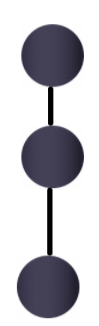
\includegraphics[scale = 0.7]{q1a.png}
		\end{center}
	
		{\bf Árvores binárias:} \\
		\hspace*{1cm}Seguindo a mesma lógica de uma árvore normal, ela possui em teoria os mesmos aspectos, porém, diferentemente de uma árvore normal, a árvore binária poderá apenas ter um número limitado de “galhos” (arestas/arcos) por nó, sendo o mínimo 0 (zero), e o máximo de 2 (dois). Vale salientar que o primeiro nó, pode ser chamado de outros nomes, como: “Nó pai” ou “Nó raiz”.\\ \hspace*{1cm} Outros nós, vindos da raiz principal, são chamados de: “Nó filho”, e esses filhos podem ter outros filhos, mas não se tornam um Nó pai, tendo exceção da regra, apenas se o nó pai for removido da árvore, daí então um dos filhos tomam o lugar de Nó raiz. Também ressaltando que nós diretamente ligados entre um nó pai e suas “folhas” (últimos nós que não possuem filhos) são chamadas de “Nós internos”, e a própria folha de “Nó externo”.
	
		\begin{center}
			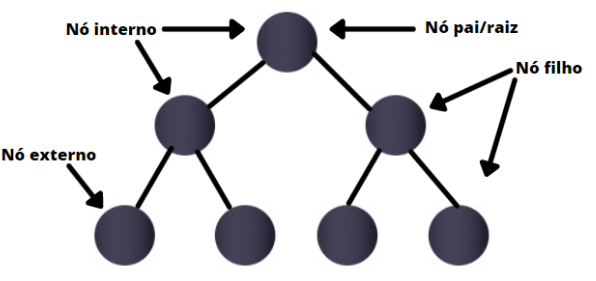
\includegraphics[scale = 0.7]{q1a1.png}
		\end{center}
	
	{\bf Árvores binárias de busca:} \\
	\hspace*{1cm} A árvore binária de busca segue a mesma regra que a árvore binária normal, tendo seu diferencial a forma em que seus filhos são alocados na árvore principal, de forma ordenada por classificação. \\
	\hspace*{1cm}Pensemos em um exemplo com letras, onde a letra K é a raiz, e adicionamos a letra A nesta árvore, no alfabeto, A vem antes do K, logo, é alocada no espaço à esquerda da raiz principal, facilitando o processo de busca da letra. Adicionando as letras, P, N e R, seguindo esta ordem, todas do lado direito (pois no alfabeto são encontradas após o K), seguindo a regra de um nó poder ter no máximo dois filhos, o P recebe o lugar ao lado do K, o N é alocado como filho do P do lado esquerdo, por vir antes da letra P no alfabeto. O R é alocado à direita, pois vem após a letra P, seguindo a mesma linha de raciocínio. 
	É possível demonstrar com a figura abaixo:
	
		\begin{center}
			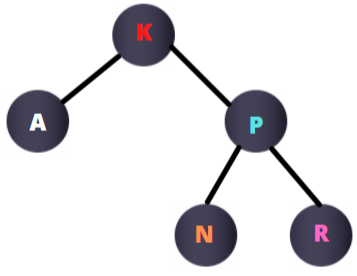
\includegraphics[scale = 0.7]{q1a2.png}
		\end{center}
	
	
	{\bf Árvores de busca balanceadas:} \\
	\hspace*{1cm}  As árvores de busca balanceadas seguem os princípios das anteriores, com mais uma regra a ser acrescentada a sua particularidade, a altura da árvore (o nível e quantidade de galhos que possuem em uma escala vertical) não pode ultrapassar 1, basicamente é a mesma coisa de ver uma árvore de verdade possuindo um lado totalmente maior que outro, por ter sido podada errado. Nesta árvore AVL nós a “podamos” para deixar seus lados iguais com uma diferença mínima (de no máximo 1) entre seus lados.
	 \\ \hspace*{1cm}Como mostrado no exemplo abaixo, podemos dizer que esta árvore é balanceada, e de busca, pois segue os requisitos de números maiores à direita, menores à esquerda, e uma diferença entre altura de apenas 1:
	
		\begin{center}
			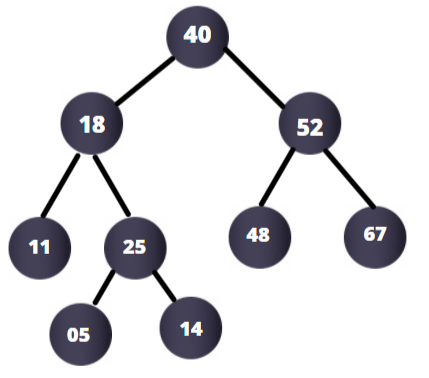
\includegraphics[scale = 0.7]{q1a3.png}
		\end{center}
	
	\newpage
	
		    \item {\bf Explique sobre as formas de se percorrer uma árvore binária. Dê um exemplo para cada uma das formas citadas.}\\ \\
		{\bf Pré-ordem:} \\
	\hspace*{1cm} A primeira forma de percurso a ser abordada consiste em fazer com que os nós de uma árvore binária sejam visitados de maneira recursiva, primeiramente apresentando o elemento (item) do nó visitado (começando pela raiz), em seguida passando para o elemento do nó filho à subárvore à esquerda e por último, passa para o elemento do nó filho à subárvore direita. A figura abaixo ilustra esse percurso:

	
		\begin{center}
			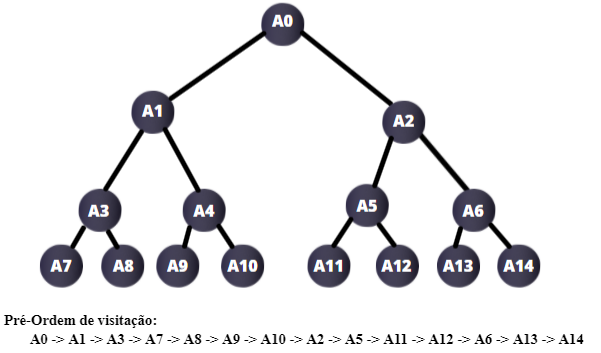
\includegraphics{q1bPreOrdem.png}
		\end{center}

	Pseudo-Código do percurso Pré-Ordem:
	\begin{lstlisting}

	void pre_ordem ( ArvRaiz *raiz ){
	
		if ( raiz != NULL ){
			printf("%d\n", raiz -> num);
			pre_ordem ( raiz -> esquerda );
			pre_ordem ( raiz -> direita );
		}
	}
	
	\end{lstlisting}

\newpage
	
		{\bf Em-ordem:} \\
	\hspace*{1cm}Nessa forma de percurso também consiste em fazer com que os nós de uma árvore binária sejam visitados de maneira recursiva, porém diferentemente da pré-ordem, é inicialmente passado para o elemento do ultimo nó filho à subárvore da esquerda, em seguida é apresentado o elemento (item) do nó visitado, volta para o seu pai, e visita o outro nó ao lado do primeiro elemento printado (o irmão do primeiro elemento apresentado), e por último, passa para o ultimo elemento do nó filho à subárvore direita. A figura abaixo ilustra essa forma de percurso:

	
		\begin{center}
			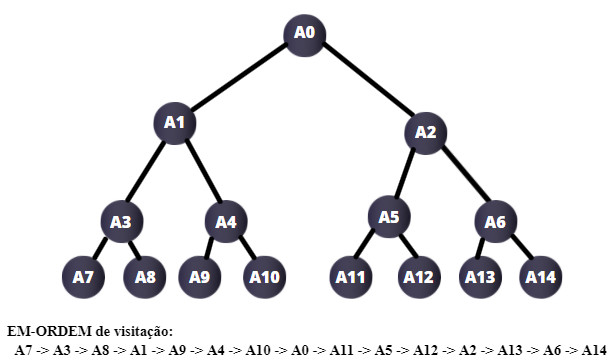
\includegraphics{q1bEmOrdem.png}
		\end{center}

	Pseudo-Código do percurso Em-Ordem:
	\begin{lstlisting}
	void em_ordem ( ArvRaiz *raiz ){

		if ( raiz != NULL ){
			em_ordem ( raiz -> esquerda );
			printf ("%d\n", raiz -> num );
			em_ordem ( raiz -> direita );
		}
	}


	\end{lstlisting}

\newpage

		{\bf Pós-ordem:} \\
	\hspace*{1cm}No percurso pós-ordem de uma árvore binária, os nós também são visitados de maneira recursiva, diferentemente da pré-ordem e em-ordem, se inicia passando para o elemento do nó filho à subárvore à esquerda, posteriormente, passa para o elemento do nó filho à subárvore direita (primeiro as folhas, depois seus pais) e por fim apresenta o elemento(item) do nó visitado. A figura abaixo ilustra essa forma de percurso:

		\begin{center}
			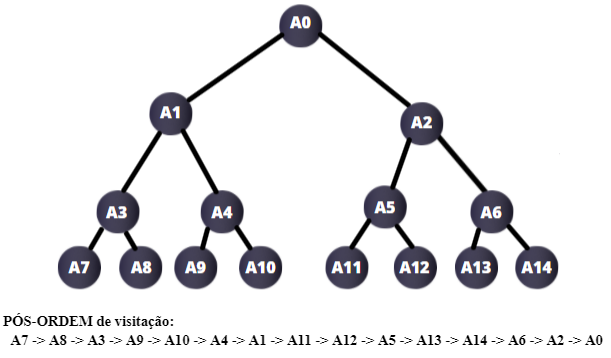
\includegraphics{q1bPosOrdem.png}
		\end{center}

	Pseudo-Código do percurso Pós-Ordem:
	\begin{lstlisting}
	void pos_ordem ( ArvRaiz *raiz ){

		if ( raiz != NULL ){
			pos_ordem ( raiz -> esquerda );
			pos_ordem ( raiz -> direita );
			printf ("%d\n", raiz -> num );
		}
	}


	\end{lstlisting}

\newpage
	
	 	   \item  {\bf Implemente um TAD para árvores binárias de busca para armazenar chaves inteiras. Esse TAD deve ter as seguintes operações: criação da árvore, inserção de um nó, remoção de um nó, busca de um nó, mostrar árvore e retornar o número de folhas da árvore. Faça um programa para testar o seu TAD.} \\

\begin{center}
Código arvere.h
\end{center}

			\begin{lstlisting}
			
// ============== Inicio .h ==================//
#ifndef ARVERE_H
#define ARVERE_H

#include <stdio.h>
#include <stdlib.h>

typedef struct arvorebin ArvBin;

struct arvorebin {
	int num;
	ArvBin* dir;
	ArvBin* esq;
};

typedef struct raiztot ArvRaiz;

struct raiztot {
	ArvBin* raiz;
};

ArvRaiz *cria_arv ( );	//cria uma arvore do 0

static ArvBin* busca ( ArvBin *r, int val );	//busca um numero especifico na arvore toda

ArvBin * raizbusc ( ArvRaiz* rz, int val );	//passa a base da arvore e seus dados

static ArvBin* inseregalho (ArvBin* r, int val); //insere um valor (chave) na arvore

void arvinsere (ArvRaiz* r, int val);	//passa os dados para inseregalho

static ArvBin * removegalho (ArvBin * r, int val);

ArvBin * raizremove (ArvRaiz * r, int val);	//chama removegalho e retira um no da arvore

int folhas (ArvBin* a);	//retorna a quantidade de folhas

int folhasRaiz (ArvRaiz *ar);

static void imprime (ArvBin* r);

void imprimeraiz (ArvRaiz* raiz);	//printa toda a arvore

#endif
// ============== Fim .h ==================//

			\end{lstlisting}


\begin{center}
Código arvere.c
\end{center}

			\begin{lstlisting}

// ============== Inicio .c ==================//
#include "arvere.h"

ArvRaiz *cria_arv ( ){
	
	ArvRaiz* a = ( ArvRaiz * ) malloc ( sizeof ( ArvRaiz ) );	//aloca espaco na memoria
	
	a -> raiz = NULL;
	puts("Raiz criada!\n");		//feedback se a arvore foi criada com sucesso
	return a;
}

static ArvBin* busca ( ArvBin *r, int val ) {
	
	if ( r == NULL )	//se nao tiver, nao busca
		return NULL;
	else
		if ( val > r -> num )		//se o valor for maior do que o no atual, passa para direita
			return busca ( r -> dir, val );
			
		else if ( val < r -> num ) 	//se o valor for menor do que o no atual, passa para esquerda
			return busca( r -> esq, val );
			
		else 
			return r;
}

ArvBin * raizbusc ( ArvRaiz* rz, int val ) {

	return busca ( rz->raiz , val );	

}

static ArvBin *inseregalho (ArvBin* r, int val){

	if ( r == NULL ) { 

		r = ( ArvBin* ) malloc(sizeof ( ArvBin ) ); 
		
		r-> num = val;
		r-> dir = NULL;
		r-> esq = NULL;
			
	}else if ( val < r -> num ) {

		r-> esq = inseregalho( r -> esq, val );
	}
	else if ( val > r-> num ) { 

		r-> dir = inseregalho( r -> dir, val );
	}
	return r;	

}

void arvinsere (ArvRaiz* r, int val){

	r -> raiz = inseregalho ( r->raiz ,val );

}

static ArvBin * removegalho (ArvBin * r, int val){
	
	if (r == NULL)	//vazio, nao tem oq remover

		return NULL;

	else if (r-> num > val)	//vai para esquerda (dependendo do valor)

		r-> esq = removegalho ( r->esq , val );

	else if (r-> num < val)	//vai para direita 

		r-> dir = removegalho ( r->dir, val );
		
	else { 
	
		//nao possui filhos
		if (r-> esq == NULL && r-> dir == NULL) {
	
	 		free (r);
			r = NULL;
		}
		//possui filhos apenas na direita
		else if (r-> esq == NULL) {
	
			ArvBin* t = r;
			r = r-> dir;
			free (t);
	
		}
		//possui filhos apenas na esquerda
		else if (r-> dir == NULL) {
	
			ArvBin* t = r;
			r = r-> esq;
			free (t);
	
		}

		else { // possui os dois filhos
	
			ArvBin* f = r-> esq; //cria uma arvore binaria f (sem raiz) e passa o valor da esquerda para ela
		
			while (f-> dir != NULL) { //enquanto direita for diferente de de nulo, pegue o valor mais a direita
	
				f = f-> dir;
			}
	
			r-> num = f-> num; //troca de dados
			f-> num = val;
			r-> esq = raizremove (r->esq ,val); //remove o valor escolhido
		}
	}
	return r;
}

ArvBin *raizremove (ArvRaiz * r, int val){
	
	r -> raiz = removegalho ( r->raiz, val); //chama a funcao anterior passando a raiz da principal (que possui dados ArvBin: esq, dir, valor)
	return r-> raiz;
}

int folhas (ArvBin* a){
	
	if ( a -> esq == NULL && a->dir == NULL ) //se nao tiver filhos, eh uma folha, logo, soma +1.
	
		return 1;
	
	else if ( a->esq != NULL && a -> dir == NULL)		//se esquerda tem filhos, ir afundo na esquerda ate chegar na folha
	
		return folhas(a->esq);
	
	else if ( a -> esq == NULL && a -> dir != NULL ) 	//se direita tem filhos, ir afundo na direita ate chegar na folha
	
		return folhas ( a -> dir );
	
	return folhas( a -> esq ) + folhas( a -> dir );	//retorna valores a esquerda e a direita da raiz principal.
} 

int  folhasRaiz (ArvRaiz *ar){
	
	return folhas( ar -> raiz );
	
}

static void imprime (ArvBin* r){ 	//utilizando preordem (comecando do primeiro ponto que eh a raiz)
	printf("<");
	
	if (r != NULL) {

		printf("%d", r -> num);
		
		imprime( r-> esq );
				
		imprime( r-> dir );
	}
	printf(">");
}

void imprimeraiz (ArvRaiz* raiz){

	return imprime(raiz -> raiz);
}

// ============== Final .c ==================//
	\end{lstlisting}

\newpage

\begin{center}
Main.c
\end{center}
\begin{lstlisting}
// ============== Inicio Main ==================//
#include "arvere.h"

int main() {
	
	ArvRaiz *arvereraiz = cria_arv (); 	//criacao de arvore
	
	arvinsere ( arvereraiz, 125); 	//insere dados aleatorios apenas para teste
	
	arvinsere ( arvereraiz, 200); 
	arvinsere ( arvereraiz, 165); 
	arvinsere ( arvereraiz, 67);  
	arvinsere ( arvereraiz, 156); 
	arvinsere ( arvereraiz, 53);  
	arvinsere ( arvereraiz, 27);  
	
	
	imprimeraiz(arvereraiz);	//impressao de dados
	
	printf("\nNumero de folhas: %d \n", folhasRaiz(arvereraiz));	//folhas presentes na arvore
	
	if(raizbusc(arvereraiz, 27))	//retorna 1 ou 0, se 1, achou, se 0, nao.
		puts("\nAchou numero 27!!");
	else
		puts("\nNada do numero 27 nessa!");
	
	raizremove(arvereraiz, 156);	//remocao de valor
	puts("\nRemovendo numero 156...");	//feedback
	
	imprimeraiz(arvereraiz);	//impressao da arvore inteira
	
	puts("\n\nInserindo valores: 232, 173, 130.\n\nEm teoria, esses valores criam 2 folhas a mais!\n");
	
	arvinsere ( arvereraiz, 232); 	//a partir daqui se repete o q ocorreu acima
	arvinsere ( arvereraiz, 173); 
	arvinsere ( arvereraiz, 130); 
	
	imprimeraiz(arvereraiz);
	
	printf("\nNumero de folhas: %d \n", folhasRaiz(arvereraiz));
	
	puts("\n\nInserindo valores: 61, 82, 97, 70.\n\nEm teoria, esses valores criam 3 folhas a mais! \n");
	
	arvinsere ( arvereraiz, 61); 
	arvinsere ( arvereraiz, 82); 
	arvinsere ( arvereraiz, 97); 
	arvinsere ( arvereraiz, 70); 
	
	imprimeraiz(arvereraiz);
	
	printf("\nNumero de folhas: %d \n", folhasRaiz(arvereraiz));
	
	
	return 0;
}
// ============== Final Main ==================//
\end{lstlisting}

Seu output no sistema foi:

			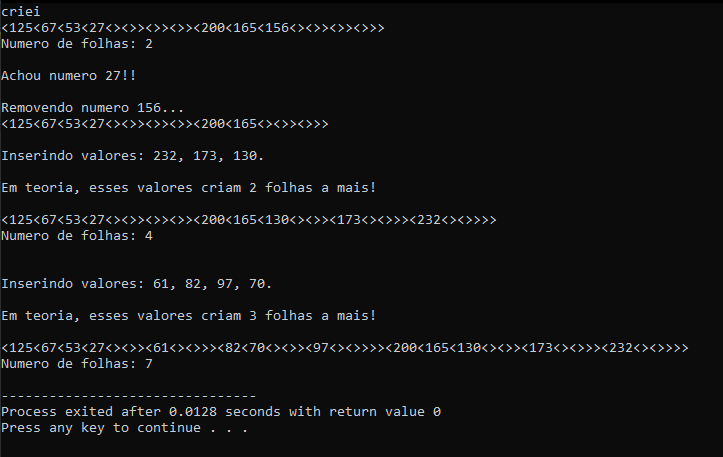
\includegraphics[scale = 0.8]{codigo.png}

O "criei" na primeira linha é um debug para confirmar que a raiz principal foi criada.
Logo em seguida, fiz o programa inserir os valores 125, 67, 53, 27, 200, 165, 156. \\ \\
Como é visível, é possivel notar como eles estão separados, numeros maiores que 125 ao lado direito, numeros menores ao lado esquerdo. A medida que o código avança, pesquiso pelo numero 27, e ele é achado, é possivel pesquisar qualquer número.
\\
A remoção do numero 156 foi um sucesso, e ele não faz mais parte da árvore. O resto é apenas repetição e amostragem de folhas. Demonstração abaixo: \\ \\

\begin{figure}
    \centering
    \begin{minipage}{0.45\textwidth}
        \centering
        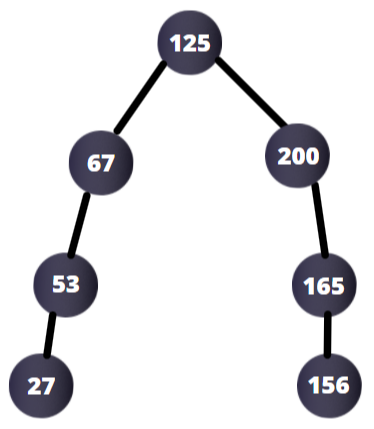
\includegraphics[scale = 0.6]{codigobin1.png}
        \caption{Estado inicial}
    \end{minipage}\hfill
    \begin{minipage}{0.45\textwidth}
        \centering
        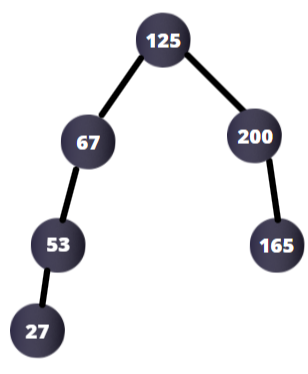
\includegraphics[scale = 0.686]{codigobin2.png}
        \caption{Remoção do 156}
    \end{minipage}
\end{figure}

\begin{figure}
    \centering
    \begin{minipage}{0.45\textwidth}
        \centering
        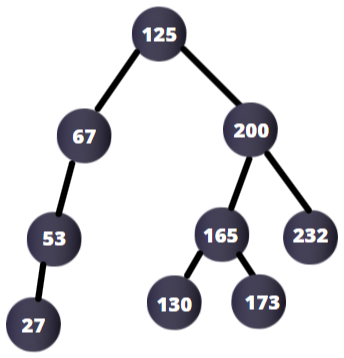
\includegraphics[scale = 0.565]{codigobin3.png}
        \caption{Adição do 232, 173, 130.}
    \end{minipage}\hfill
    \begin{minipage}{0.45\textwidth}
        \centering
        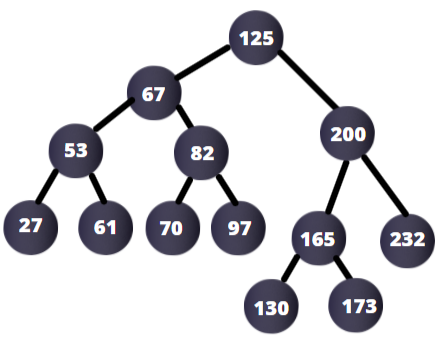
\includegraphics[scale = 0.565]{codigobin4.png}
        \caption{Adição do 61, 82, 97, 70.}
    \end{minipage}
\end{figure}

\newpage

	\item
{\bf Explique e dê exemplos sobre as operações aplicadas em árvores binárias de busca para que estas se tornem árvores AVL. }\\ \\ 
\hspace*{1cm} Após a inserção ou remoção de algum elemento que tenha desequilibrado na distribuição dos elementos, o conceito de rotação de nós numa árvore objetiva o restabelecimento do balanceamento da árvore. \\
\hspace*{1cm}O  conceito de árvore AVL, já apresentado anteriormente, fica melhor explicado com as duas figuras abaixo, uma vez que, na figura 1 a inserção da chave 36 na árvore a torna desbalanceada, pois a diferença de altura entre as subárvores do nó raiz é superior a 1. Na figura 2 é mostrado o restabelecimento do balanceamento com a rotação de nós utilizando rotação à direita.

		\begin{center}
			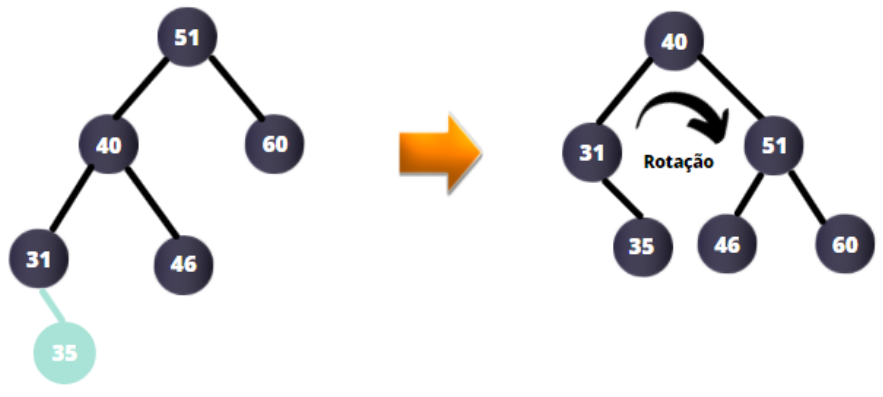
\includegraphics[scale = 0.6]{q1a4.png}
			{\small A esquerda, figura 1, a direita, figura 2.}
		\end{center}

	{\bf Código Rotação à direita:} \\
		\begin{center}
			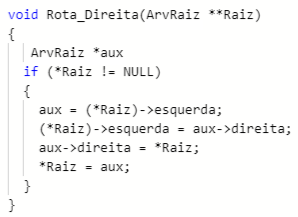
\includegraphics[scale = 0.85]{rotadireita.png}
		\end{center}	
{\small O aux aponta o nó filho à esquerda da raiz da subárvore, o nó filho à direita de aux passa a ser o nó filho à esquerda da raiz, a variável do tipo ArvRaiz ** Raiz passa a ser o nó filho à direita de aux, aux passa a ser a nova Raiz da subárvore.}

\newpage
{\bf Rotação à esquerda} \\
\hspace*{1cm} Neste tipo de rotação, o nó raiz da subárvore é deslocado para a posição de seu nó filho à esquerda, que, por sua vez, continua a ser o nó filho à esquerda do nó deslocado. O nó filho à esquerda do nó filho à direita da raiz é deslocado para ser o nó filho à direita do nó raiz deslocado. O nó filho à direita do nó raiz ocupa o seu antigo lugar, passando a ser a nova raiz.

		\begin{center}
			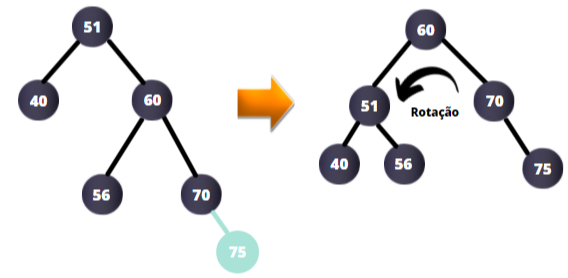
\includegraphics[scale = 0.85]{rotaesqim.png}
		\end{center}	
	
	{\bf Código Rotação à esquerda:} \\
		\begin{center}
			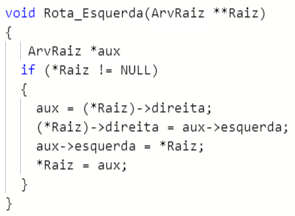
\includegraphics[scale = 0.85]{rotaesquerda.png}
		\end{center}	
{\small Basicamente uma repetição do código de rotação apresentado anteriormente, sendo a principal diferença, inicialmente a variável auxiliar (aux) aponta o nó filho à esquerda da raiz da subárvore, e vice-versa.}

\newpage

\hspace*{1cm} Também existe a rotação dupla, em que é utilizada as aplicações anteriores, onde há uma diferença na altura da árvore AVL (maior que 1 de altura, como explicado em tópicos anteriores), porém, a primeira operação, ao invés de modificar a árvore toda, ela modificará apenas a parte de baixo do lado com maior altura.\\ Após a primeira operação, é executada uma rotação no sentido oposto à anterior. Para melhor entendimento, segue abaixo uma ilustração: 

		\begin{center}
			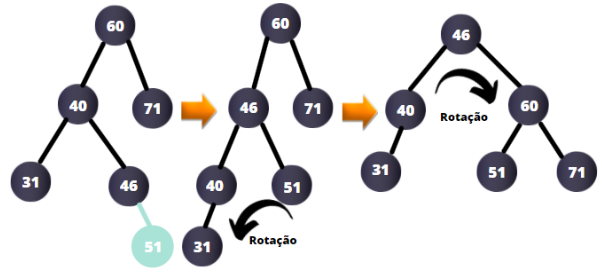
\includegraphics[scale = 0.85]{rotadupl.png}
		\end{center}	

\hspace*{1cm}Com isso, é possível chegar na conclusão que Árvores AVL utilizam como base as Árvores Binárias e suas operações são a mesmas, apenas com a adição da constante verificação de diferença em altura da árvore e balanceamento. \\ Logo, estas são funções que checam se um lado da árvore está a uma diferença maior que 1 (ou menor que -1)  comparada a nós adjacentes, e se estiver, ela utilizará uma ou mais funções apresentadas anteriormente em busca de um equilíbrio em altura e mantendo a ordem das chaves presentes anteriormente.

	\end{enumerate}

\newpage

\section{Questão 2}

	\begin{enumerate}[a)]
		\item {\bf Construa a matriz de adjacências para este grafo.} \\ \\

		\begin{center}
			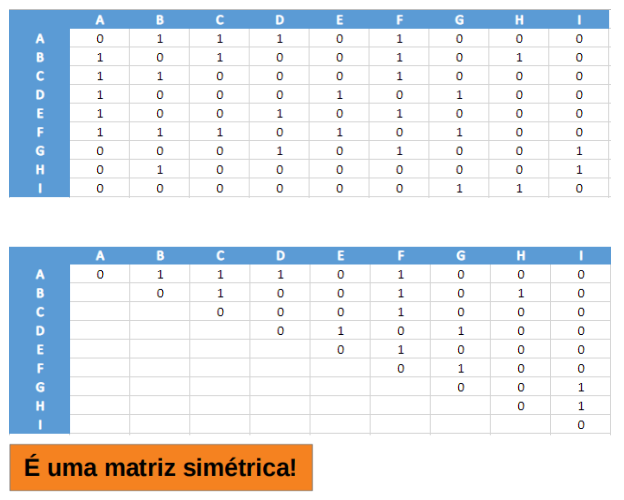
\includegraphics[scale = 0.7]{q2a.png}
		\end{center}

\newpage

		\item {\bf Começando do nó A, explique como o grafo é percorrido em profundidade.} \\ \\

		Seguindo por ordem alfabética: \vspace{0.3 cm}

Ordem de visitação com retorno: A, B, C, F, E, D, G, I, H, I, G, D, E, F, C, B, A. \\ 
Ordem de visitação sem retorno: A, B, C, F, E, D, G, I, H. \\ 


		\begin{center}
			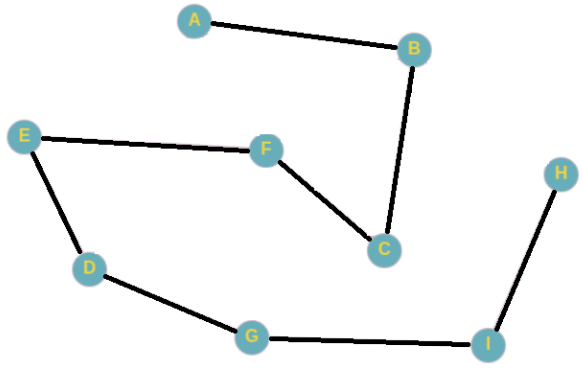
\includegraphics[scale = 0.7]{q2b.png}
		\end{center}

A imagem acima já mostra o caminho percorrido pelo grafo (via profundidade, indo cada vez mais fundo e por ordem alfabética) indo pelo caminho disponível, dada a forma em que o grafo estava distribuído.

\newpage

\item {\bf Começando do nó A, explique como o grafo é percorrido em largura.} \\ \\


Ordem de visitação (Numerado por ordem de visitação):  1.A, 2{DFCB}, 3.E, 4.G, 5.H,  6.I \\ 
Ordem de visitação (Apenas o caminho percorrido): A - D - F - C - B - E - G - H - I \\ \\
Ordem de exclusão e adição (Já visitados e quais eles adicionam à lista acima): \vspace*{0.1cm}
{\small (legenda: NAN - Não adiciona ninguém, AD - Adiciona algum à lista)}

 A (//AD - D, F, C, B//), \\
 D (//AD - E, G//), \\
 F (NAN), \\
 C (NAN), \\
 B (//AD - H//), \\
 E (NAN), \\
 G (//AD - I), \\
 H (NAN), \\
 I (NAN). \\

		\begin{center}
			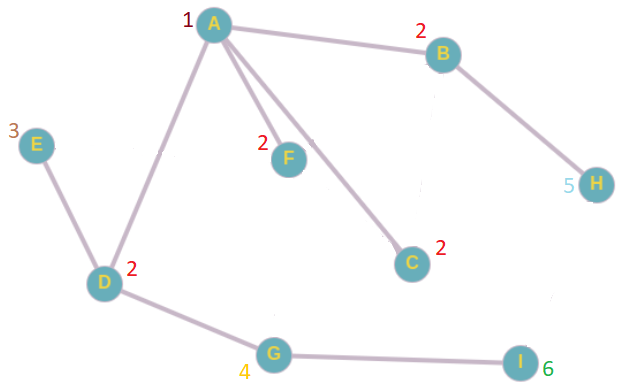
\includegraphics[scale = 0.7]{q2c.png}
		\end{center}
Primeiramente, o inicio a partir do nó A, segue para todos os nós de valor 2 (em vermelho na imagem). Após isso, o D aponta para o E, e retorna ao D, depois indo para a letra G E a letra I. A letra B irá para a letra H.

\newpage

	\item
{\bf Construa o pseudo-código para algoritmo de Bellman-Ford e explique o seu funcionamento através de um exemplo.} \\ \\

\hspace*{1cm}O algoritmo de Bellman-Ford basicamente consiste em uma estratégia mais simples para se encontrar os caminhos mínimos a partir de um vértice para qualquer outro vértice de um grafo. O algoritmo faz relaxar todas as arestas do grafo, repetindo até que não precise mais fazer uma relaxação, o número máximo de iterações do algoritmo de Bellman-Ford pode ser apresentado como é V - 1. \\ Uma implementação do algoritmo de Bellman-Ford é mostrado logo abaixo. \\ \\

{\bf Pseudocódigo do Algoritmo de Bellman-Ford} \\ \\

\begin{lstlisting}

void Bellman_Grafo (Grafo* g, int s){

	inicializa(g); // associa o custo infinito para todos os vertices 
	
	g->v[s]. custo = 0.0;	//Custo de s = 0
	
	for (int k = 1; k<g->n; ++k) { 	//quantidade de nos
	
	  for (int i = 0; i<g->n; ++i) {
	
	    for ( Aresta* a = g->v[i]. lista; a!= NULL; a = a-> prox) {
	
	       int j = a->v;
	
	     relaxa(g, i , j, a-> custo); 	//se o ligamento entre o no i e j for menor que o custo da aresta a, substitui o custo pelo o custo minimo
	              }
	        }
	    }
}

\end{lstlisting}

\newpage

{\bf Exemplo do percurso de um Grafo utilizando o algoritmo de Bellman-Ford} 

	\begin{minipage}{0.6\textwidth}
  		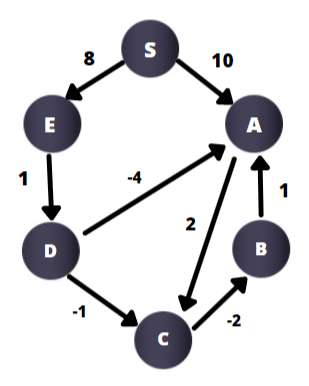
\includegraphics[scale = 0.9]{q2d.png}
	\end{minipage}
	\begin{minipage}{0.3\textwidth}	
\hspace*{1cm}	S sempre é 0 pois é a partida, primeiramente S passa para o A , que tem como valor 10, logo em seguida, do valor A para o valor C, valor de A=10 para C=2 é 10+2=12, de C para o B menos 2 ,sendo assim 12-2 = 10 então o valor de B é 10, de E para o D é 9, pois de S para o E é 8, e de E para D é 1,isto é, 8+1=9, concluindo que D = 9. \\ A tabela abaixo mostra o resultado da primeira iteração.
	\end{minipage} \\

	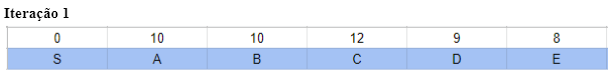
\includegraphics[scale = 0.9]{q2d1.png}

\vspace*{1cm}
\hspace*{1cm}	 S sempre é 0 pois é a partida, agora pelo o lado esquerdo do S, S para E é valor 8, então E continua  no mesmo valor, do E  para D é 8+1 = 9, também continua o mesmo valor, o D pode partir para A e para o C, se partir para A, temos D= 8+1 = 9, então  9-4 = 5, agora A= 5, no D para o C temos o valor -1, sendo assim D= 8 +1= 9,  de D para C é 9-1= 8, mudando, agora C = 8. \\ A tabela abaixo mostra o resultado da segunda iteração. \\ \\
	
	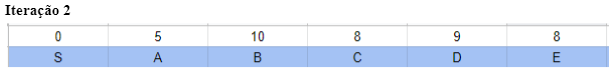
\includegraphics[scale = 0.9]{q2d2.png}

\newpage

\vspace*{1cm}
\hspace*{1cm}	Começando com S=0, A vai continuar valendo 5 pois o valor 10 é maior, do A para o C, A= 5+2 = 7, uma vez que 7 menor que 8, o valor de C vai ser substituído por 7, agora C=7, de C para B é 7 -2 , mudando o valor de B para 5, já que 5 é menor que 10, D e E continua os mesmos valores. \\ A tabela abaixo mostra o resultado da terceira iteração. \\ \\

	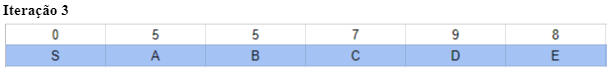
\includegraphics[scale = 0.9]{q2d3.png}

\vspace*{1cm}
\hspace*{1cm}	Precisamos checar se tem algum valor que possa ser substituído, S para A é 10, sendo assim o valor de A não muda, continua 5, valor do A para C é 5+2 = 7 ,  continua também o mesmo valor para C, vamos do S pelo outro lado, 8+1 = 9 , e 9-1= 8 não é menor que 7, continua o mesmo valor de B = 5 porque o percurso de A à B é A valendo 5+2 = 7, então 7 - 2 do B é igual a 5, por outro lado, para o D não tem mais outro caminho, vai ser sempre o 9, pois 8+1 = 9, e E é sempre valendo 8, pois também não tem outro caminho. \\ A tabela abaixo mostra o resultado da quarta iteração. \\ \\


	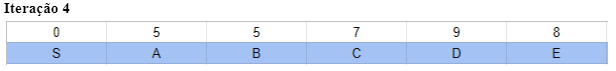
\includegraphics[scale = 0.9]{q2d4.png}

\newpage

	\item
	{\bf Construa o pseudo-código para o algoritmo de Dijkstra e explique o seu funcionamento através de um exemplo. }

\vspace*{0.5cm}
\hspace*{1cm} O algoritmo de Dijkstra procura otimizar a busca pelo caminho mínimo priorizando as arestas a serem relaxadas, porém tentando relaxar apenas as arestas que pertencem a uma “frente de avanço” do algoritmo, a partir do vértice origem. \\ \\

{\bf Pseudocódigo do Algoritmo de Dijkstra}

\begin{lstlisting}
static int extrai_minimo (Grafo* g){ 	 //Passa o grafo como parametro

    int iminimo = -1;

       for (int i=0; i<g->n; ++i) {

          if (g->v[i]. cor == cinza ) { 	//Verifica se a frente de avanco com o vertice tem o custo minimo

                   if (iminimo <0 || g->v[i]. custo < g->v[iminimo]. custo) 	//Verifica qual vertice tem o custo minimo
                               iminimo = i;

              }
       }
      return iminimo;
}

\end{lstlisting}

\newpage

\begin{lstlisting}

void Dijkstra_grafo (Grafo* g, int s, int t) { 	 //Passa o garfo, passa s como o no inicial, passa t(vertice de destino) como parametro
      int i;

      inicializa(g);

      g->v[s]. custo = 0.0 ;

      g->v[s]. cor = cinza ; 		// Marca s com cinza como frente de avanco

while ((i= extrai_minimo(g))>=0) { 	//Verifica com o vertice de custo minimo para ser o avanco

        g->v[i]. cor = preto ; // Marca i com preto e o vertice que foi processado

         if (i == t)

           break ; 	// Para se ja chegou ao destino

     for ( Aresta* a=g->v[i]. lista; a!= NULL; a=a-> prox) {

            if (g->v[a->v]. cor != preto ) { 		// se caso o vertice nao foi processado, relaxa a aresta

               relaxa(g,i,a->v,a-> custo); 

               g->v[a->v]. cor = cinza ; 	// Marca o vertice v com cinza como frente de avanco

                          }

                      }

             }

     }
\end{lstlisting}

\newpage

{\bf Exemplo do percurso de um Grafo utilizando o algoritmo de Dijkstra: } \\ \\

		\begin{center}
			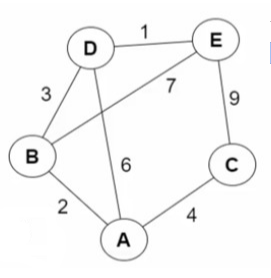
\includegraphics[scale = 1]{q2e.png}
		\end{center}

{\bf Passo 1:} \\

Para ser possível encontrar o percurso de menor distância, o primeiro passo é começar com A, que tem ligação com o B , C , D , porém não tem ligação com E. \\ Dessa forma, a tabela 1 abaixo ilustra o primeiro passo. \\

		\begin{center}
			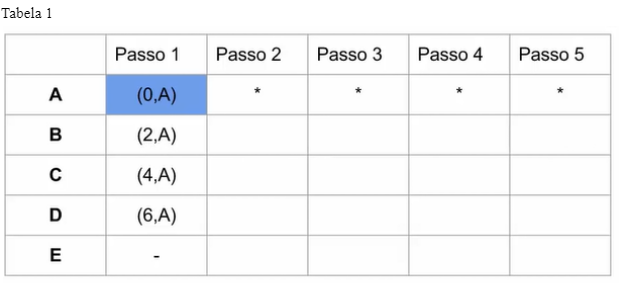
\includegraphics[scale = 0.9]{q2e1.png}
		\end{center}

\newpage

{\bf Passo 2:} \\

O segundo passo é observar qual é o menor percurso do Passo 1,  é possível notar que de A para B é 2, sendo assim, preenchendo a segunda coluna do Passo 2 com B= (2,A). Partindo de B, como não é possível ir de B a C, repete o valor de C do Passo 1, a terceira coluna do Passo 2 é C = (4,A), de B para D tem distância 2, somando com 3 do B à D, a quarta coluna do Passo 2 é igual a D = (5,B) , sendo menor que D=(6,A) do Passo 1. De B para E é uma distância de 9, pois 2+7 = 9, terminando de completar a última coluna do Passo 2  E=(9,B). \\ A tabela 2 abaixo ilustra o segundo passo. \\


		\begin{center}
			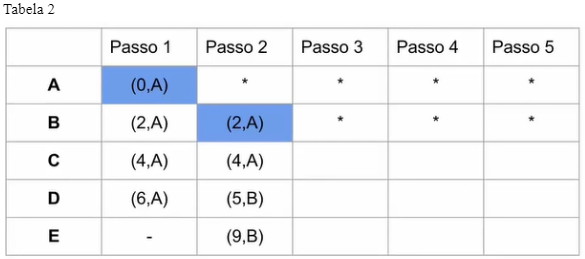
\includegraphics[scale = 0.9]{q2e2.png}
		\end{center}

\newpage

{\bf Passo 3:} \\

Seguindo para o terceiro passo, nota-se que C=(4,A) é o menor valor, portanto a terceira coluna do Passo 3 é C = (4,A),  uma vez que C não está ligado a D, repetimos o menor valor de D, ou seja, a quarta coluna do Passo 3 é D(5,B), o percurso de C para E é 4 + 9 = 13, sendo assim, 13 é maior que o valor de E = (9,B), então mantém o E=(9,B) do Passo 2, ou seja  a última coluna do Passo 3 é  E= (9,B).  \\ A tabela 3 abaixo ilustra o terceiro passo. \\

		\begin{center}
			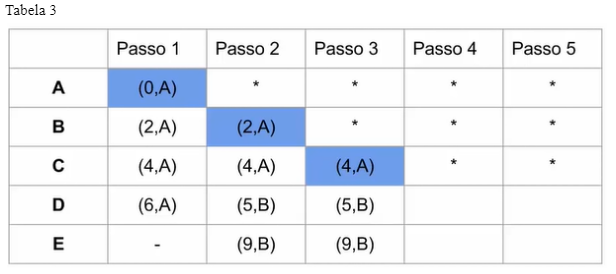
\includegraphics[scale = 0.9]{q2e3.png}
		\end{center}

\newpage

{\bf Passo 4:} \\

Avançando para o quarto passo, o menor valor do Passo 3 é D= (5,B), dessa forma, a quarta coluna do Passo 4 é D = (5,B), a menor distância para E é pelo percurso D à E, isto é, 5 + 1, a última coluna do Passo 4 é E=(6,D). \\ A tabela 4 abaixo ilustra o quarto passo. \\ \\

		\begin{center}
			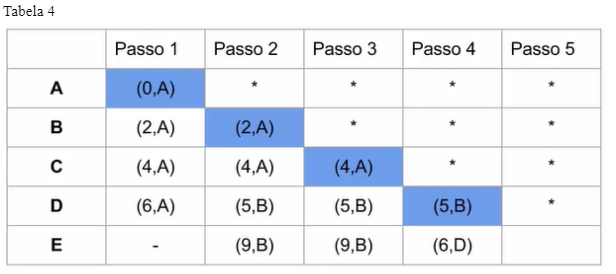
\includegraphics[scale = 0.9]{q2e4.png}
		\end{center}

\newpage

{\bf Passo 5:} \\

Para finalizar, nota-se que só existe um caminho do Passo 4, E = (6,D), concluindo assim, que a última coluna do  Passo 5 é  E= (6,D). \\ A tabela 5 abaixo ilustra o quinto e último passo. \\

		\begin{center}
			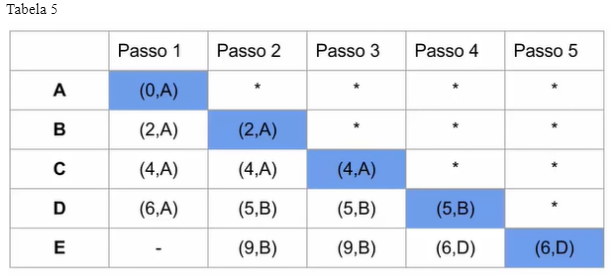
\includegraphics[scale = 0.9]{q2e5.png}
		\end{center}

	\end{enumerate}
\end{document}
